\chapter{Review and Improvements to Statistical Methods in Neutrino Astronomy}\label{chapter:methods}
Point source searches in neutrino astronomy are essentially weighted clustering analyses: each event is determined by a set of coordinates (right ascension, declination, angular error, and time), and a weight (energy), and the task is to determine if high weight points are clumped beyond what is expected purely from statistical fluctuations. Most attempts to do this make use of a similar approach, using data-driven background estimation and a likelihood-based estimator of clustering. This section outlines the general framework of such an analysis, as well as several variants of the likelihood-based clustering estimator that is commonly used. \color{red}In the simplest case, only spatial clustering is examined, and temporal information is excluded entirely ("time-integrated" analyses), however it can be additionally interesting to explore the possibility of temporal clustering of events as well, increasing the dimensionality of the clustering problem by one. Later in this section we introduce an improved method for fitting ensembles of spatial and temporal clusters of events ("flares") to characterize the data, which is an improvement over existing methods which only make use of information from the most significant flare. This fills in the methodological gap that can be seen in table~\ref{tab:stresults}. \color{black}

\section{Clustering Analysis Outline for an Arbitrary Test Statistic}
There are many ways of constructing a test statistic in neutrino astronomy, in addition to a variety of types of clustering to look for (for example, clustering near various source catalogs, clustering in space and time, clustering with weights according to source/event energy weights, clustering about an extended spatial feature such as the galactic plane). However, almost all clustering analyses in this area share several features in their construction:

\begin{enumerate}
    \item A test statistic is formulated, which ideally tests the degree of clustering of astrophysical events near a particular source candidate location. This test statistic is typically a likelihood-based test statistic of a form similar to that which is described in the following section, however this test statistic is often modified to reflect the specifics of the clustering hypothesis being tested. 
    \item A background test statistic distribution is calculated using maps generated from data that has the right ascension values of events randomized. This destroys any clustering that may have already been present, providing an excellent representation of the null hypothesis (a purely diffuse astrophysical neutrino flux with no spatial or temporal clustering). As this background estimation is data-driven, it is robust against unknown backgrounds that may be present in the sample. Scrambling the data does not affect the sample event content, and consequently the underlying distributions of event declination, energy, and arrival time are unchanged. 
    \item Alternative hypothesis test statistic distributions may be obtained from simulations of signal events. If the analysis is not sensitive to the total astrophysical neutrino flux, simulated events can simply be added to the background maps generated above. If the analysis is sensitive to the total astrophysical flux, then more sophisticated methods (such as moving existing events instead of injecting new events) may be required. Once maps containing signal have been generated, they can be used both to characterize the performance of the analysis, as well as compute upper limits in the event of a null result.
    \item The performance of the test statistic being used is typically evaluated using the \textit{sensitivity} and/or \textit{discovery potential}. The \textit{sensitivity} refers to the amount of signal that needs to be injected before 90\% of the test statistic distribution is greater than the median of the background test statistic distribution. Similarly the \textit{discovery potential} refers to the amount of signal that needs to be injected before 50\% of the test statistic distribution is greater than the $N\sigma$ significance threshold in the background test statistic distribution ($N$ is typically either 3 or 5, but can be other values. This is typically clarified by stating that the value reported is the "N-sigma discovery potential"). "Amount of signal" is intentionally ambiguous here, as different analyses are sensitive to different types of signal. The sensitivity and discovery potential can be cast in terms of any number of variables that may be relevant to a particular analysis. For example, in the time-integrated case, these values are often reported as a flux, however time-dependent analyses may report a fluence, and analyses sensitive to source populations may even report their sensitivity as a curve in the space of source density and source luminosity. 
    \item The test statistic is calculated for the observed data sample, and this observed test statistic is compared to the distribution generated in step 2 to calculate a p-value. This p-value is then used to either accept/reject the null hypothesis of no clustering.
\end{enumerate}

\begin{figure}[h]
\centering
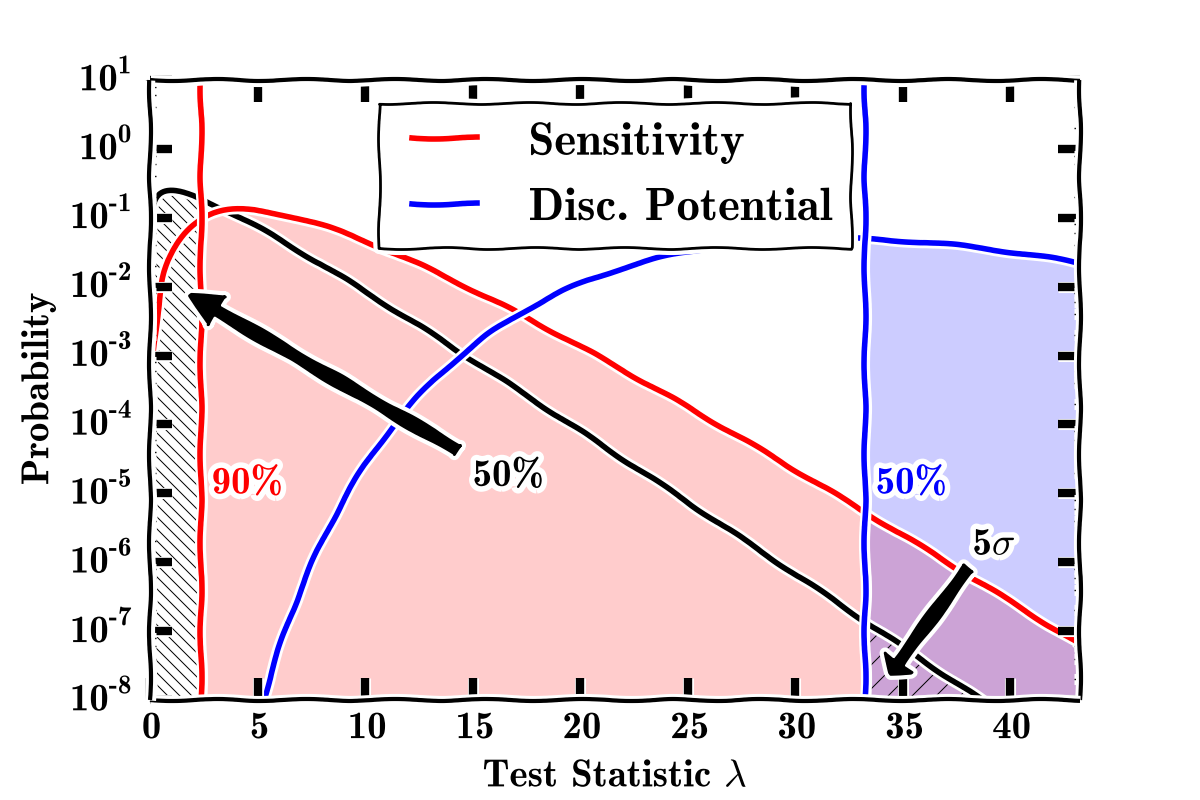
\includegraphics[width=0.8\textwidth]{figs/sens_discpotential.png}
\caption{A toy plot showing the definitions of sensitivity and discovery potential. \cite{Reimann:2019zby}}
\label{fig:angres}
\end{figure}

\section{Unbinned Time Integrated Methods}
Astrophysical point sources may be distinguished from the atmospheric neutrino background by way of clustering: if astrophysical sources are present in the data, events should be clustered near one another, while atmospheric events are expected to be isotropically distributed. Additionally, since high energy neutrino events are more likely to be astrophysical in origin, clustering of these events can be an even stronger indicator of the effect of neutrino point sources in the data. In short, we would like to construct a test statistic that reflects these observations. This can be done by way of a likelihood-based test statistic, using a likelihood composed of signal and background PDFs that describe the spatial and energy properties of events relative to a source candidate location. For a neutrino sample composed of $N$ total events, the likelihood of the data for some number of signal (clustered astrophysical) events, $n_s$ is (eq. \ref{psllh})\cite{Braun_2010}:

\begin{equation}
    \mathcal{L}(n_s, \gamma) = \prod_{i=1}^{N}[\frac{n_s}{N}S_i+(1-\frac{n_s}{N})B_i]
    \label{psllh}
\end{equation}

Where here, $S_i$ and $B_i$ are PDFs that describe the spatial and energy distributions of signal and background events relative to the source candidate location. $S_i$ and $B_i$ are themselves composed of spatial and energy components (eq. \ref{spaceEcomponents_sig} and \ref{spaceEcomponents_bg}). 

\begin{equation}
    S_i = R(r_i) \times \mathcal{E}(E_i, \delta_i|\gamma)
    \label{spaceEcomponents_sig}
\end{equation}
\begin{equation}
    B_i = \frac{1}{\Omega}\times \mathcal{E}(E_i,\delta_i|Atm_{\nu})
    \label{spaceEcomponents_bg}
\end{equation}

Note that the source spectral index, $\gamma$, enters as a free parameter in the energy portion of the signal PDF. 

For the background PDF, the construction is relatively straightforward: background events originate from all directions equally, so the only effect that produces anisotropies is the detector acceptance. Since the IceCube detector acceptance does not vary as a function of right ascension, we can define $B_i$ for a particular declination band to simply be $1/\Omega$, where $\Omega$ is the solid angle of a declination band centered on the source candidate declination. Similarly, the background energy PDF can be obtained by measuring the energy distribution of observed events as a function of declination. 2D histograms of event counts as a function of declination and event energy are assembled, and these distributions are then splined to create PDFs that can be used to evaluate $B_i$ for events at an arbitrary declination and energy. 

\begin{figure}[h]
\centering
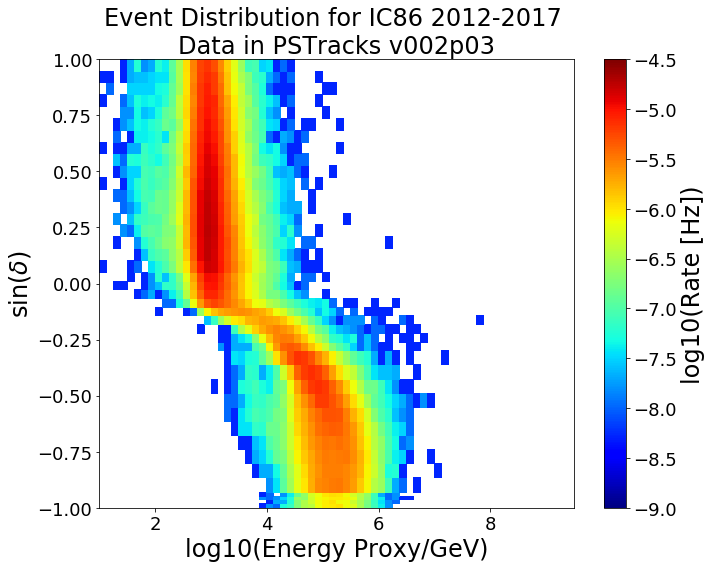
\includegraphics[width=0.4\textwidth]{figs/psv2_edec.png}
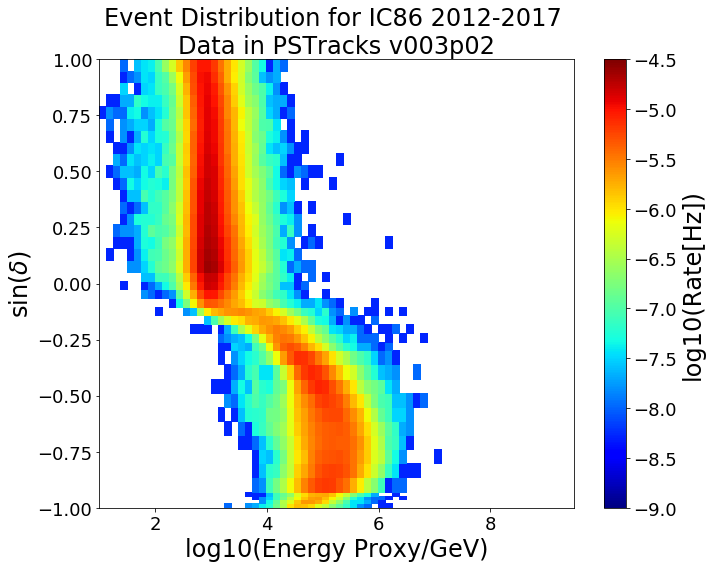
\includegraphics[width=0.4\textwidth]{figs/psv3_edec.png}
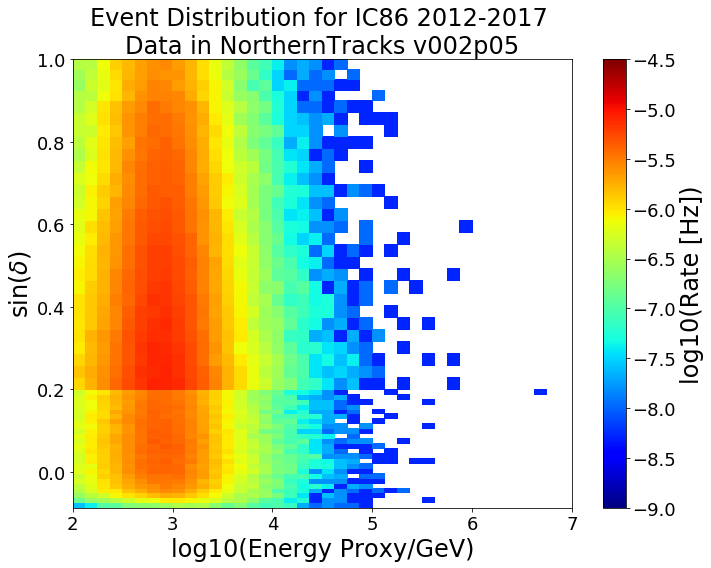
\includegraphics[width=0.4\textwidth]{figs/nt_edec.png}
\caption{2D histograms of declination and energy proxy for the 3 IceCube track event samples discussed in this document: PointSourceTracks v002p03 (left), PointSourceTracks v003p02 (right) and NorthernTracks v005p02 (bottom). Splines of these distributions are used as background PDFs in the clustering likelihood described in equation~\ref{psllh}\cite{10yrpublicdata}. The NorthernTracks dataset is restricted to the northern sky, and additionally the splines associated with this dataset use finer binning near the horizon, hence the seeming dicontinuity near $\sin(\delta)=0.2$}
\label{fig:DecEnDist}
\end{figure}

Unlike background events, signal events are expected to be clustered near the source candidate location. For this reason, the spatial component of the signal PDF, $R(r_i)$, is assumed to be a 2-D gaussian centered on the source candidate location (eq. \ref{sigspacepdf}):

\begin{equation}
    R(r_i) = \frac{1}{2\pi\sigma_{i}^2} e ^{-\frac{r_i^2}{2\sigma_i^2}}
    \label{sigspacepdf}
\end{equation}

Where $r_i$ is the angular distance between the $i$th event and the source candidate location and $\sigma_i$ is the event angular error.  

The energy component of $S_i$ is obtained from simulation: Simulated events are weighted according to a particular astrophysical spectral index, creating a 2D PDF describing the sum of simulated event weights as a function of declination and energy. These maps are then divided by the background PDF described above to create a map describing the "signalness" of events at a particular energy and declination, given a spectral index. As these maps are created for a range of spectral index values (typically ranging between $\gamma=1$ and $\gamma=4$), a 3-D PDF of event energy, declination, and spectral index hypothesis results from this process. This is precisely the function $\mathcal{E}(E_i, \delta_i|\gamma)$ that enters the likelihood, and can be used to fit for $\gamma$, given events observed at declination $\delta$ with energy $E_i$.  

\begin{figure}[h]
\centering
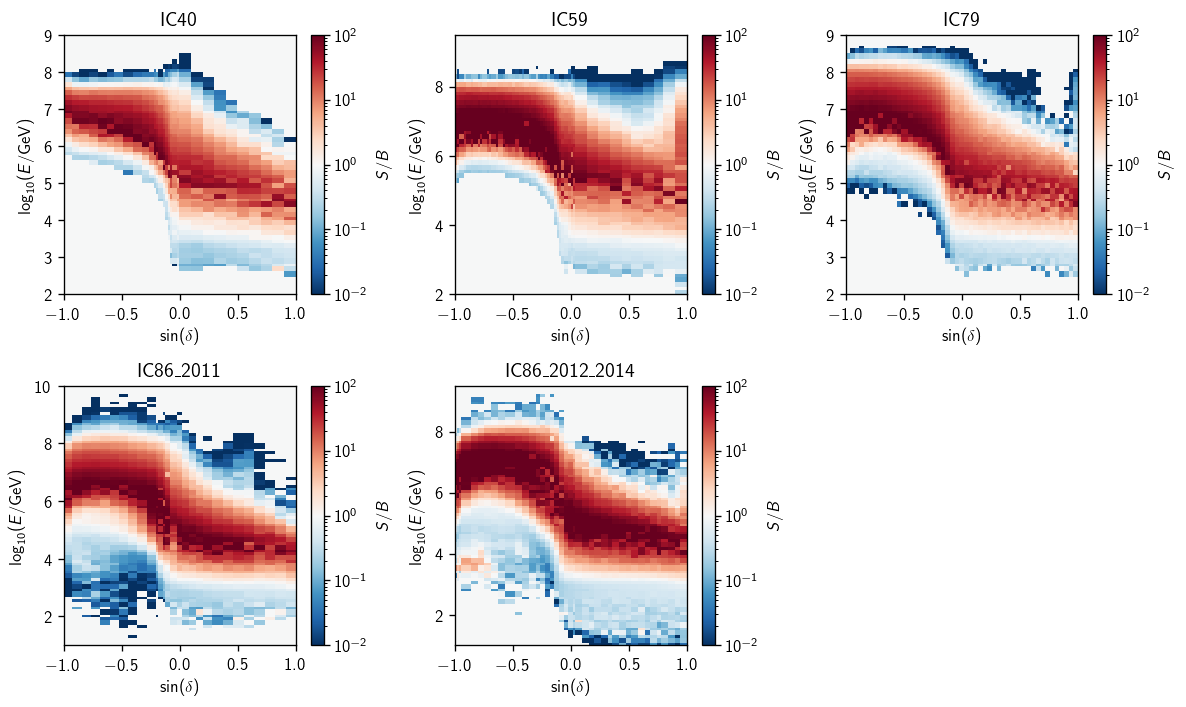
\includegraphics[width=0.8\textwidth]{figs/sig_hists.png}
\caption{Signal PDFs associated with a $\gamma=2.0$ spectral index hypothesis, assembled from PSTracks v002p03. Similar PDFs are constructed for spectral indices ranging from $\gamma=1.0$ to $\gamma=4.0$, thereby constructing a 3-D PDF that can be used in the point source likelihood.}
\label{fig:SigPDf}
\end{figure}

The likelihood described in eq. \ref{psllh} can be maximized as a function of $\n_s$ and $\gamma$, resulting in best fit parameters $\hat{n_s}$ and $\hat{gamma}$. We can then compute a test statistic for a given data sample from the likelihood ratio (\ref{psts}):

\begin{equation}
    TS = -2 \log \frac{\mathcal{L}(n_s=0)}{\mathcal{L}(\hat{n}_s, \hat{\gamma})}
    \label{psts}
\end{equation}

This test statistic can then be used in the generalized framework described in the sections above to test the hypothesis of spatial clustering of astrophysical neutrino events near a particular source location. 

This framework can be applied to multiple locations at once, and the results combined by summing the individual test statistics calculated at each location (note that this is equivalent to calculating the product of the likelihoods). This process is often referred to as "source stacking", and can be used to improve sensitivity to dim sources, provided there are multiple emitters in the source candidate list. 

Other methods of combining information across multiple source locations exist as well. In particular, the binomial test is a popular way of doing this. Give a list of source candidates and their associated p-values, we can search for the most significant combination of source candidates by employing the binomial test-statistic (eq. \ref{bitest})

\begin{equation}
    p(k) = \sum_{i=k}^{N_{eff}} \binom{N_{eff}}{i}p_k^i(1-p_k)^{N_{eff}-i}
    \label{bitest}
\end{equation}

Where $p(k)$ is the p-value associated with combining the results of the $k$ most significant sources, $N_{eff}$ is the effective number of trials (often simply equal to the total number of source candidates), and $p_k$ is the p-value of the $k$th most significant source. The minimum of p(k) can then be computed and treated as a test statistic, to obtain a p-value associated with the best-fit number of sources ($k_{min}$) in a particular catalog. 


\section{Unbinned Time-Dependent Methods}
In addition to being clustered in space, astrophysical neutrino events may also be clustered in time (a neutrino "flare"). Accounting for this temporal clustering may allow us to identify sources that are insignificant under a corresponding time integrated analysis. Studying the temporal variation of source candidates can also inform us of the specifics of the source dynamics of particle production, as the time scale of observed flares is related to the physical scale of the astrophysical objects in which particle production is occurring. This method was used in ~\cite{txs_archival} to identify the 2014 neutrino flare candidate with a significance of $3.5 \sigma$. 

\subsection{Optimizing for a Single Flare}
We can modify our time-integrated likelihood to account for potential temporal clustering as well by simply appending a temporal PDF to the existing PDFs that describe the spatial and energy components of the analysis (eq. \ref{tmodllh1}, \ref{tmodllh2}):

\begin{equation}
    S_i = R(r_i) \times \mathcal{E}(E_i, \delta_i|\gamma) \times \mathcal{T}(t_i)
    \label{tmodllh1}
\end{equation}

\begin{equation}
    B_i = \frac{1}{\Omega}\times \mathcal{E}(E_i,\delta_i|Atm_{\nu}) \times \frac{1}{\delta T}
    \label{tmodllh2}
\end{equation}

Where $\delta T$ is the full livetime of the sample, and the associated temporal background PDF is $1/\delta T$, as the background event rate should be constant. In practice, this is assembled in a data-driven manner by measuring the data sample event rate in each of the 8-hour segments ("runs") that are used to segment the data. In this way, seasonal variations of the detector event rate are accounted for by the likelihood, as the flare candidates are always being compared to the local event rate in time.

\begin{figure}[h]
\centering
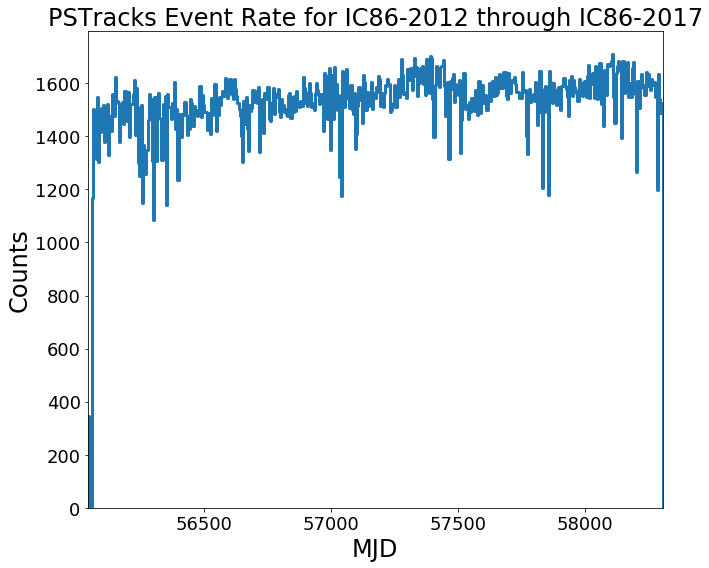
\includegraphics[width=0.8\textwidth]{figs/evt_rate.png}
\caption{The event rate of the IC86 seasons of the PointSourceTracks v3 data sample. This event rate can be used to generate a background temporal PDF in the time-dependent clustering likelihood.}
\label{fig:evt_rate}
\end{figure}

The temporal contribution to the signal PDF, $\mathcal{T}(t_i)$, can take various forms depending on the particular shape that one assumes for the time profile of flare candidates, but the most basic temporal profile can be used is a box (eq. \ref{boxflare}):

\begin{equation}
    \mathcal{T}(t_i | t_0, \Delta t) = 
    \begin{cases} 
      0 & t_i < t_0 \\
      \frac{1}{\Delta t} & t_0 \leq t_i \leq t_0+\Delta t \\
      0 & t_i > t_0 + \Delta t
   \end{cases}
   \label{boxflare}
\end{equation}

This box-shaped temporal PDF essentially asks as a mask, filtering for events that occur within the time window between $t_0$ and $t_0 + \Delta t$. The events within this time window then contribute to the likelihood in a similar manner to the time-integrated case. Note that by adding this temporal PDF to the likelihood, we have also introduced 2 new parameters that the likelihood can be maximized with respect to: $t_0$ and $\Delta T$, which describe the flare start time and duration, respectively. 

Similar to the time-integrated case, a likelihood ratio test statistic can be assembled from this likelihood, however this test statistic can be further improved in the time-dependent case by accounting for the duration of flare candidates that were scanned over (eq. \ref{psts_tdep}:

\begin{equation}
    TS = -2 \log [\frac{\Delta T}{\hat{\Delta t}}\frac{\mathcal{L}(n_s=0)}{\mathcal{L}(\hat{n}_s, \hat{\gamma}, \hat{t}_0, \hat{\Delta t}}]
    \label{psts_tdep}
\end{equation}

Where the the factor $\frac{\Delta T}{\Delta t}$ can be interpreted as a trial factor that accounts for the fact that there are significantly more short flare candidates that can be tested than long ones (e.g. there is only 1 potential flare candidate with $\Delta t = \Delta T$, but there are many flares that can be made with $\Delta t = \Delta T/100$). This factor normalizes the test statistic scale between short and long flares \cite{Braun_2010}.

In practice, this process is extremely computationally intensive due to the number of likelihood minimizations that need to be performed. This can be mitigated by seeding flares with events that already have a high probability of being signal in origin, based off their energy and arrival direction. An ensemble of seed events can be defined to the set of events with $S_i/B_i$ greater than some threshold value, where $S_i$ and $B_i$ refer to the signal and background PDF components of the time integrated likelihood (describing only the spatial and energy properties of contributing events). Typically this threshold is set to be relatively low ($S_i/B_i > 1$), however higher values can also be used if computational requirements are particularly stringent (e.g. if running over the entire sky). 

Many analyses compute the test statistic in eq. \ref{psts_tdep} for a variety of flare candidates, and then use the flare with the maximum test statistic as the "best-fit" flare. The test statistic associated with this "best-fit" flare is then compared to a distribution of "best-fit" flares obtained from the background case (generated from data scrambled in right ascension), resulting in a p-value that describes the strength of the clustering hypothesis relative the the null hypothesis of no clustering. 

In simulated signal trials, the likelihood-based flare test statistic is able to reconstruct the injected number of signal events in each flare with reasonable accuracy, and the per-flare spectral index fits show similar agreement as well. 

\begin{figure}[h]
\centering
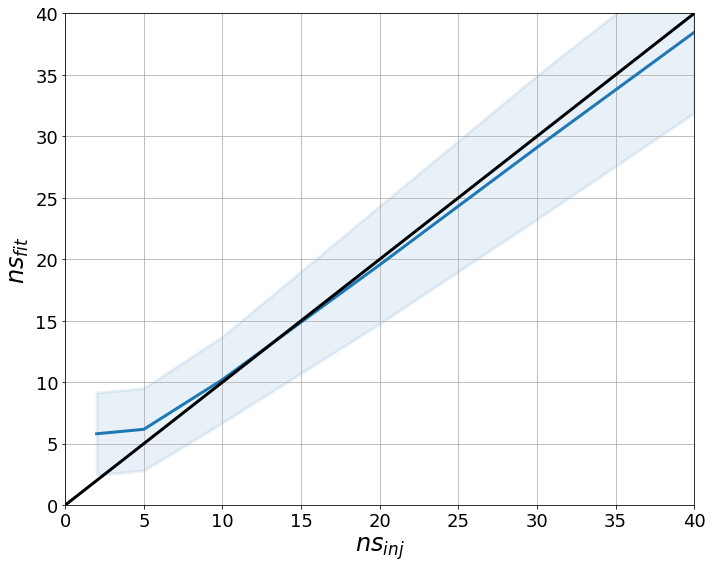
\includegraphics[width=0.4\textwidth]{figs/nsfit.png}
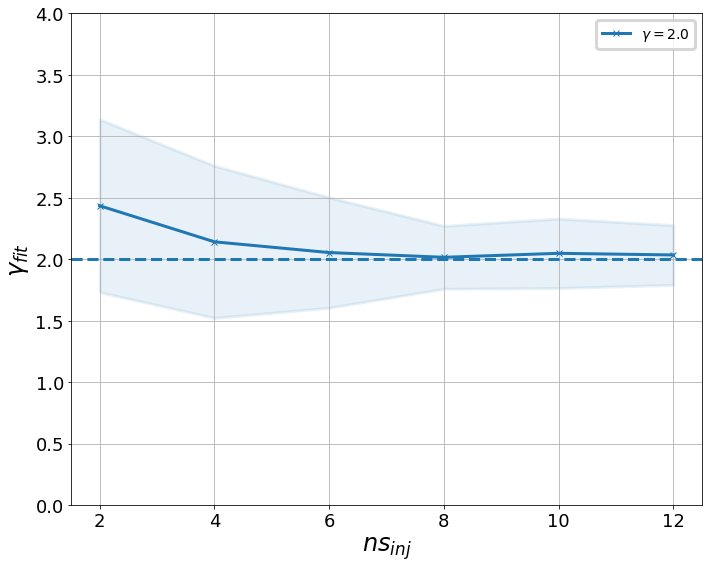
\includegraphics[width=0.4\textwidth]{figs/gamfit_2.0.png}
\caption{The best fit number of signal events in a flare, and the best fit spectral index versus the true number of signal events injected in simulated trials. On average, for flares with $> \approx 5$ events, the time-dependent likelihood is able to accurate estimate the true number of signal events.}
\label{fig:perflare_nsfit}
\end{figure}


\subsection{Improving the Search for Temporal Clustering: Fitting Ensembles of Multiple Flares}
As the IceCube detector collects more data, it becomes increasingly useful to be able to test the hypothesis of multiple neutrino flares that may have occurred at a particular location. Fitting only the largest flare is advantageous if the source flare rate is expected to be low enough that sources only flare once over the data-taking period, however if sources flare multiple times the single-flare analysis potentially misses a significant amount of useful information. \color{red}By incorporating information from multiple flares at a particular location, an analysis can be sensitive to a smaller individual flare intensity. This is analagous to spatial stacking analyses, as can be seen in table~\ref{tab:stresults}, but we have additionally improved our algorithm to stack \textit{flares} instead of just spatial source candidates. In this section we discuss the construction of this method, and the following sections describe the results of the first applications of this method to various source catalogs. \color{black}

The process of fitting multiple flares at a particular source candidate location is similar to the single-flare maximization procedure described above. Flare candidates are seeded by events with a high $S_i/B_i$ ratio near the candidate location. For each flare candidate, the test statistic described in equation \ref{psts_tdep} is calculated. Unlike the single flare case, these flare candidates are then ordered by decreasing test statistic value, and any flares that overlap in time with a different flare that itself has a higher test statistic are removed. Additionally, any flares with a test statistic $< 0$ are removed. What remains is a temporally decorrelated ensemble of flare candidates, each with $TS>0.$. This ensemble functions as a neutrino "flare curve" (similar to light curves produced by photon-based telescopes), that describes the temporal variability of the signal originating from a source candidate location. A "multi-flare" test statistic describing the significance of the temporal variability of this source candidate can then be calculated as the sum of the individual flare candidate test statistics (eq. \ref{multiflareTS}):

\begin{equation}
    \widetilde{TS} = \sum_{j=0}^{N_{flares}} TS_{j}
    \label{multiflareTS}
\end{equation}

Where here, $j$ is an index that refers to the individual flares that compose the neutrino flare curve. This test statistic can then be compared to an ensemble of similar test statistics generated from right-ascension scrambled (background) data to obtain a final p-value describing the significance of the set of flares that were fit at a particular source candidate location. 

An estimation of the total number of signal events can be obtained in a similar manner (eq. \ref{mfns}), where the total number of signal events associated with a particular source candidate is just the sum of the best-fit number of $n_s$ in each contributing flare candidate:

\begin{equation}
    \widetilde{n}_s = \sum_{j=0}^{N_{flares}} \hat{n}_{sj}
    \label{mfns}
\end{equation}

Note that this similar to time-integrated source stacking mentioned above, however instead of stacking test statistics associated with spatially distinct locations, we are instead stacking spatially and temporally distinct \textit{flares}.

The multi-flare algorithm is, in some sense, inclusive of the single flare algorithm: by fitting all the flares at a source candidate location, we have obviously also fit for the largest flare. It is thus trivial to obtain the single-flare significance once the multi-flare result is obtained. In order to do this, simply compare the highest flare candidate test statistic that was obtained with a distribution of single-flare test statistics obtained in a similar manner from background (right-ascension scrambled) data. 

In addition to calculating the local significance of the largest flare, the local significance of the other flare candidates composing the flare curve fit by the multi-flare algorithm can also be obtained in a similar manner. We can define the "local significance" of a particular flare (not necessarily the largest) to be the fraction of flares in the background distribution with $TS_j>TS_{j,observed}$. Note however, that the calculation of multi-flare significance is done in the space of $TS_j$, not the space of the corresponding local significances $p_j$. This means that the multi-flare significance is \textit{not} simply the product of the component flare $p_j$'s, as each flare is not entirely statistically independent from the others (e.g. once the largest flare is fit, the remaining available livetime in which other flares can be fit is reduced by an amount equal to the duration of the largest flare.) 

\begin{figure}[h]
\centering
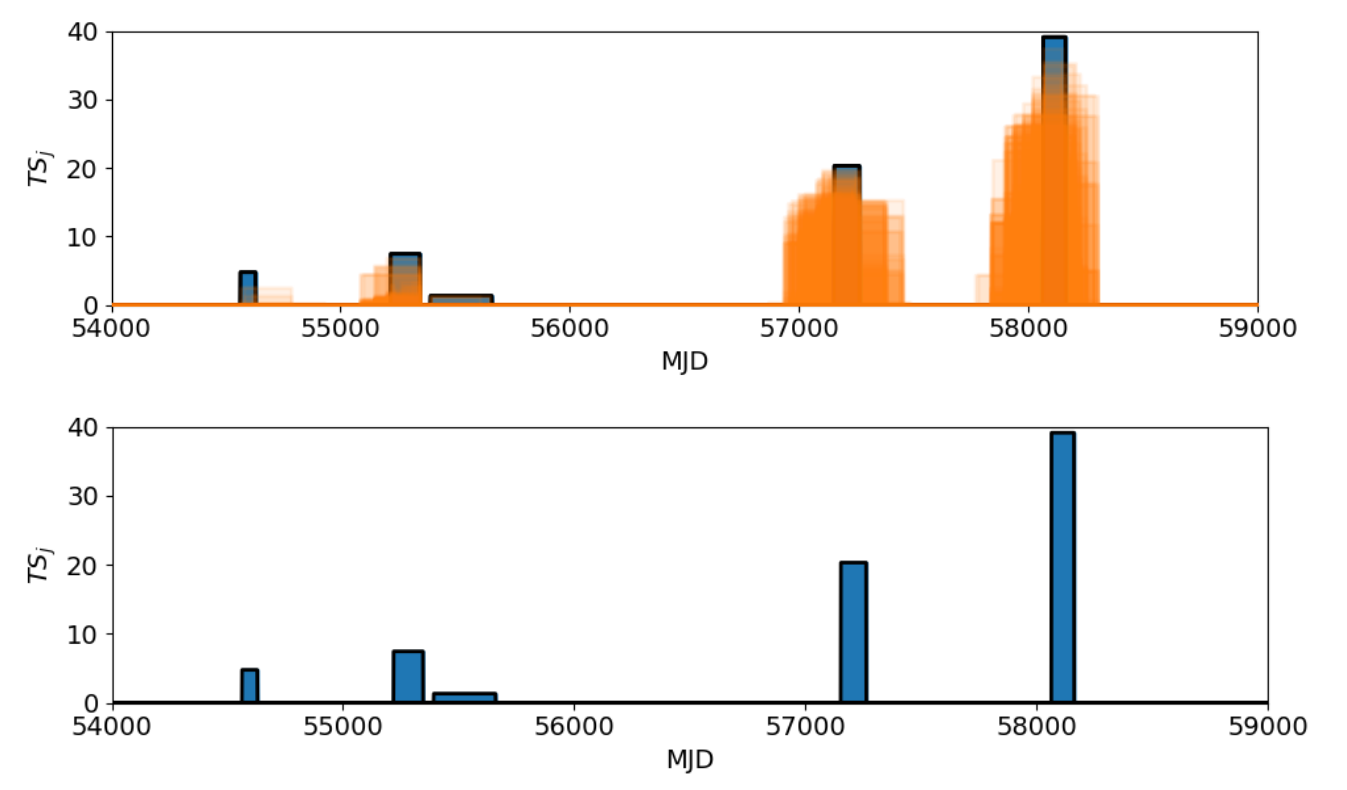
\includegraphics[width=0.8\textwidth]{figs/mf_algorithm.png}
\caption{A graphical example of the progression of the multi-flare decorrelation algorithm. Colored boxes represent flare candidates that were tested, seeded by events with high $S_i/B_i$ ratios. The height of each box corresponds to the individual flare candidate test statistic, $TS_j$. Orange flares overlap with another flare with a higher test statistic, and are consequently removed, leaving only the blue flares. The test statistics of the blue flares are then summed, and can be used for hypothesis testing of flaring neutrino emission at this source candidate location.}
\label{fig:mf_algorithm}
\end{figure}


As mentioned above, the multi-flare algorithms is particularly useful in the case of several similarly sized flares. In this case, while the single flare algorithms will identify the correct number of events in the largest flare, the estimation of the total number of signal events associated with the source candidate will be incorrect (as there is a non-negligible portion of events that belong to flares that were not identified by the single flare algorithm). By contrast, the multiflare algorithm improves the estimation of $n_s$ in the case of multiple similarly sized flares, as signal events in all flare candidates (not just the largest one) are able to contribute. This improvement is shown in figure \ref{fig:persrc_nsfit}.

\begin{figure}[h]
\centering
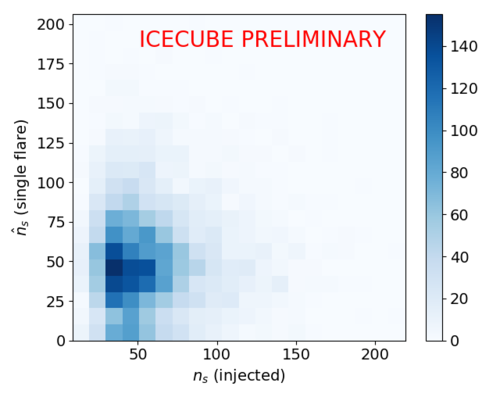
\includegraphics[width=0.4\textwidth]{figs/500px-Ns_singleflare.png}
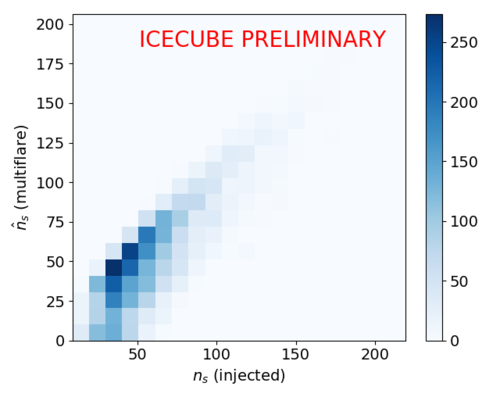
\includegraphics[width=0.4\textwidth]{figs/500px-Ns_multiflare.png}
\caption{Left: the injected vs. fit number of signal events when attempting to use the single flare algorithm to describe an ensemble of neutrino flares. Right: The same plot, but using the multiflare estimation of $n_s$ that accounts for signal events in all flare candidates.}
\label{fig:persrc_nsfit}
\end{figure}

As an example of a case where the multi-flare algorithm is advantageous, consider the case shown in \ref{fig:mf_example}, which has 3 flares injected at MJD=55246.3, 55807.4, and 57632.7 at a test location of (RA, Dec) = ($77.45^{\circ}$, $5.61^{\circ}$). The single flare method fits only the flare at MJD = 55246.3 (with TS = 22.66), while the multiflare method fits all flares together, with a multi-flare test statistic of $\widetilde{TS}$ = 60.52. While the largest individual flare only has a significance of $3.29 \sigma$, by combining information from all the flares that were fit at this location, we arrive at a multi-flare significance of $4.7 \sigma$. 

\begin{figure}[h]
\centering
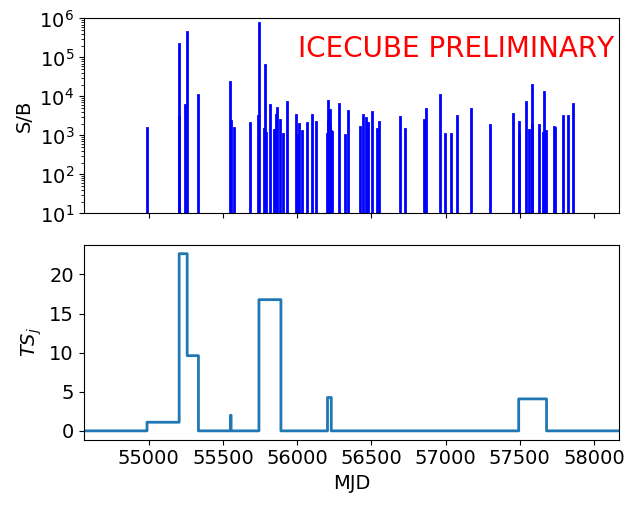
\includegraphics[width=0.45\textwidth]{figs/example_flarecurve.png}
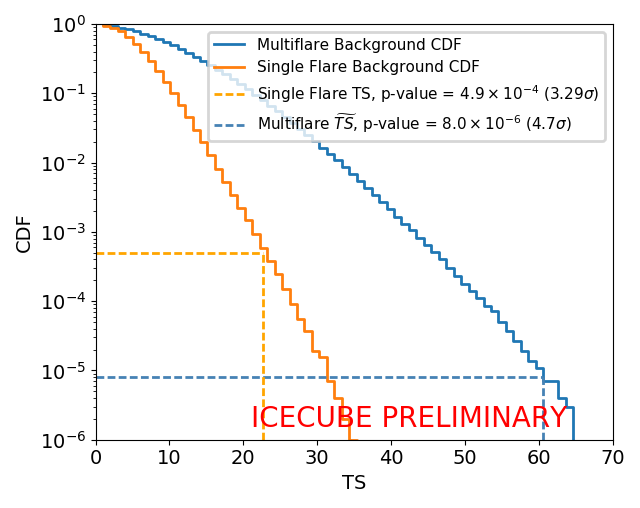
\includegraphics[width=0.45\textwidth]{figs/1src_1k_bgdist.png}
\caption{Left, top: Events that pass the $S/B$ threshold cut for generating windows, for a source located at (ra, dec) = ($77.45^{\circ}$, $5.61^{\circ}$). There are 3 injected flares, centered at MJD=55246.3, 55807.4, and 57632.7. Left, bottom: The single flare method fits only the flare at MJD = 55246.3 (with TS = 22.66), while the multiflare method fits all flares together, with a global test statistic of $\widetilde{TS}$ = 60.52. Right: The background test statistic distributions for a single source, located at declination = $5.61^{\circ}$. The background multiflare test statistic distribution is shown in blue, while the single flare method is shown in orange. The vertical lines represent the test statistics associated with the flare curve on the left The single flare p-value for this source is $4.9 \times 10^{-4}$ (3.29$\sigma$), while the multiflare p-value is $8.0 \times 10^{-6}$ ($4.7\sigma$). }
\label{fig:mf_example}
\end{figure}


